\documentclass{CUP-JNL-PPS}

%%%% Packages
\usepackage{latexsym}
\usepackage{graphicx}
\usepackage{multicol,multirow}
\usepackage{amsmath,amssymb,amsfonts}
\usepackage{mathrsfs}
\usepackage{amsthm}
\usepackage{rotating}
\usepackage{appendix}
\usepackage[authoryear]{natbib}
\usepackage{ifpdf}
\usepackage[T1]{fontenc}
\usepackage[type1,lining]{ebgaramond}
\usepackage[type1,lining]{sourcesanspro}
\usepackage{newtxmath}
\usepackage{textcomp}%
\usepackage{xcolor}%
\usepackage{hyperref}
\usepackage{lipsum}
%%%%

%\articletype{RESEARCH ARTICLE}
\jname{Perspectives on Politics}
%\artid{20}
\jyear{2021}
\jvol{4}
%\jissue{1}
\jdoi{10.1017/pps.2021.xx}
%\raggedbottom

%\usepackage{showframe}

\begin{document}

\begin{Frontmatter}

\title[Panorama Report]{CMSC426PJ2 Report}

\author{Yizhan Ao \texttt{josephao@umd.edu}}
\author{Daniel Song \texttt{dsong12@umd.edu}}
\author{Yingqiao Gou \texttt{ygou@terpmail.umd.edu}}


\abstract{Abstracts should be 250 words. It must be able to stand alone and so cannot contain citations to the paper's references, equations, etc. An abstract must consist of a single paragraph and be concise. Because of online formatting, abstracts must appear as plain as possible.}

\end{Frontmatter}


\dropcap{M}
modi minima sunt esse temporibus sint culpa, recusandae aliquam numquam
totam ratione voluptas quod exercitationem fuga. Possimus quis earum veniam
quasi aliquam eligendi.

\section[]{ANMS (Adaptive Non-Maximal Suppression)}

The goal of ANMS is to pick out the stronger corner points.
\begin{itemize}
    \item Using the cornermetric method to find all the corners of each grayscale image. 
    \item After applying imreagionalmax, we can get the strong corners in the image.
    \item Using ANMS alogrithm we can find the best pixel of each image.
    \item We analyze a 40*40 pixel square area selecting an intial 300 N-best to trial.
    \item Note: Each image may vary from sizes in real life cases 
\end{itemize}
\subsection{Shortcomings}
\begin{itemize}
    \item We specify the N-best manually choosing from 450 - 300 - 200- 100 -50
    \item The problem we think is that the level of the variable is affecting to understand the sets
    \item Even though the variable is performed well in terms of the point indication, however, we think the point may be not accurate in some points
    \item ANMS takes the amount of points which are equally distributed. However, removing some of better score points in a high score area will resulted in less accurate data in dense areas. 
    \item This could resulted to a decrease in accuracy in the feature matching and warping.
\end{itemize}

% \begin{figure}[t]%
% \FIG{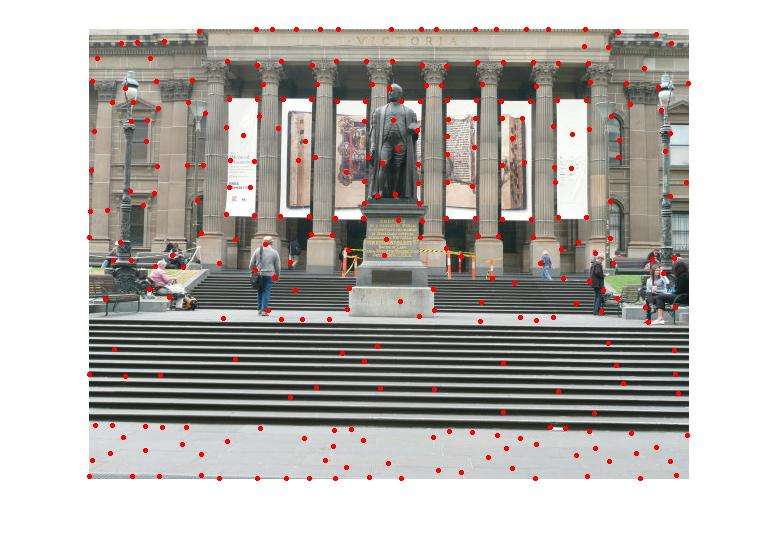
\includegraphics[width=290]{outputimages/ANMS/anms1.jpg}}
% {\caption{This is an example of caption }
% \label{fig1}}
% \end{figure}

% \begin{figure}[t]%
% \FIG{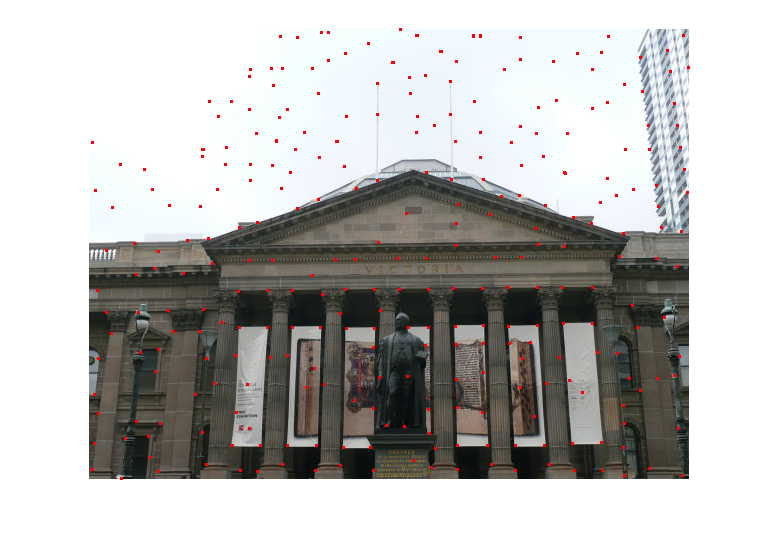
\includegraphics[width=290]{outputimages/ANMS/anms2.png}}
% {\caption{This is an example of caption }
% \label{fig2}}
% \end{figure}

% \begin{figure}[t]%
% \FIG{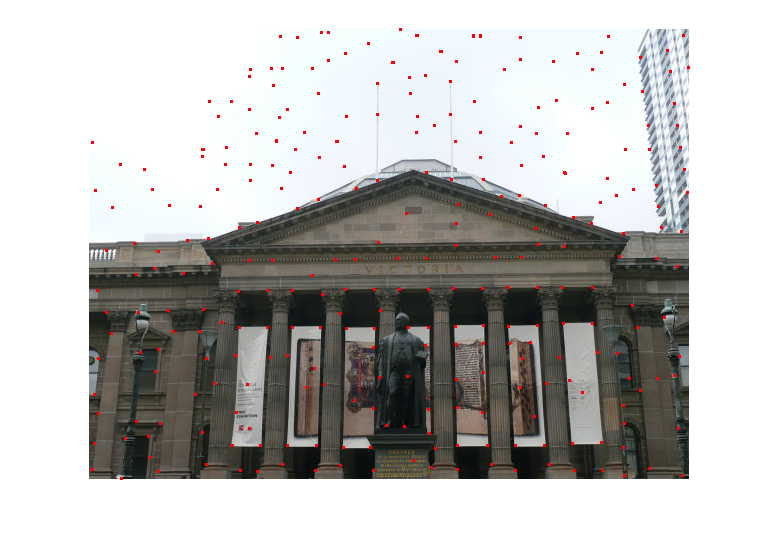
\includegraphics[width=290]{outputimages/ANMS/anms2.png}}
% {\caption{This is an example of caption }
% \label{fig2}}
% \end{figure}
\begin{center}
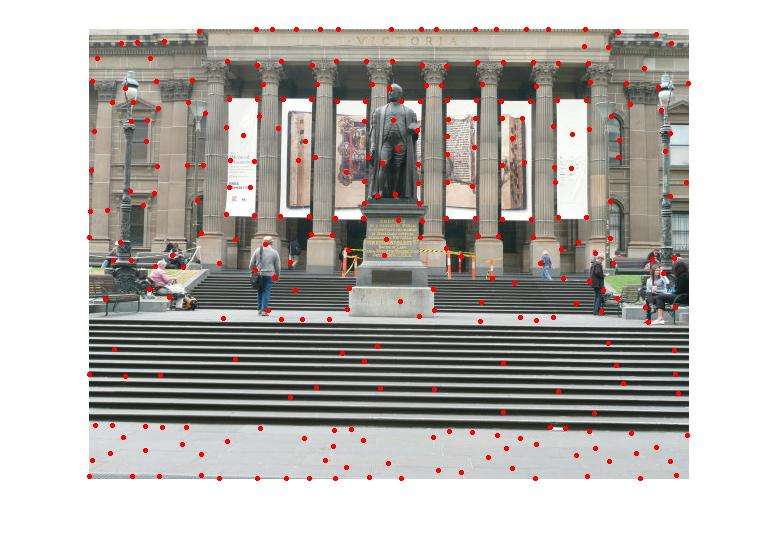
\includegraphics[width=275]{outputimages/ANMS/anms1.jpg}
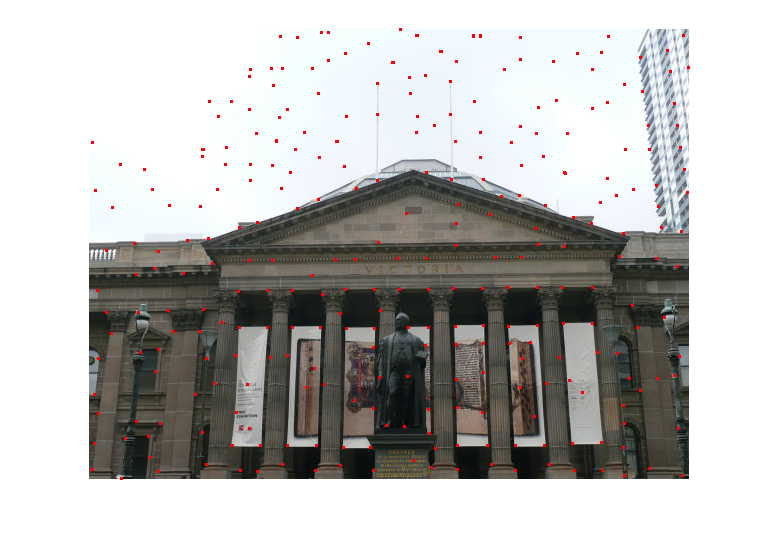
\includegraphics[width=275]{outputimages/ANMS/anms2.png}
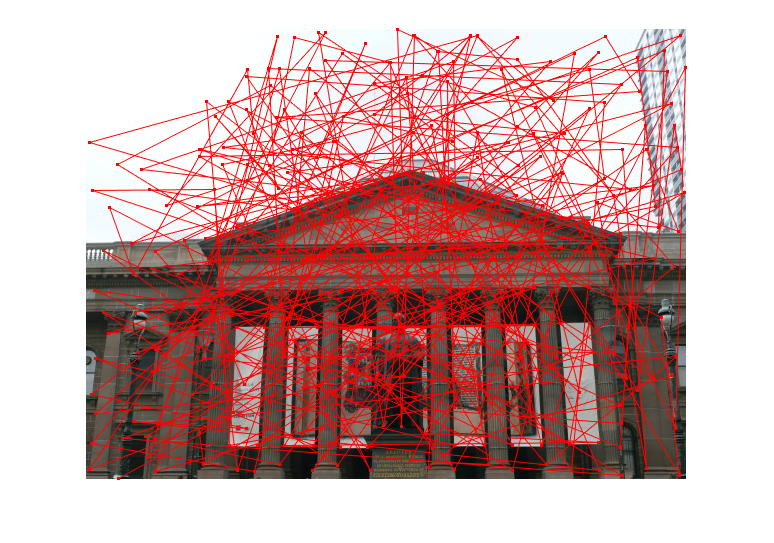
\includegraphics[width=275]{outputimages/ANMS/ANMS4.png}
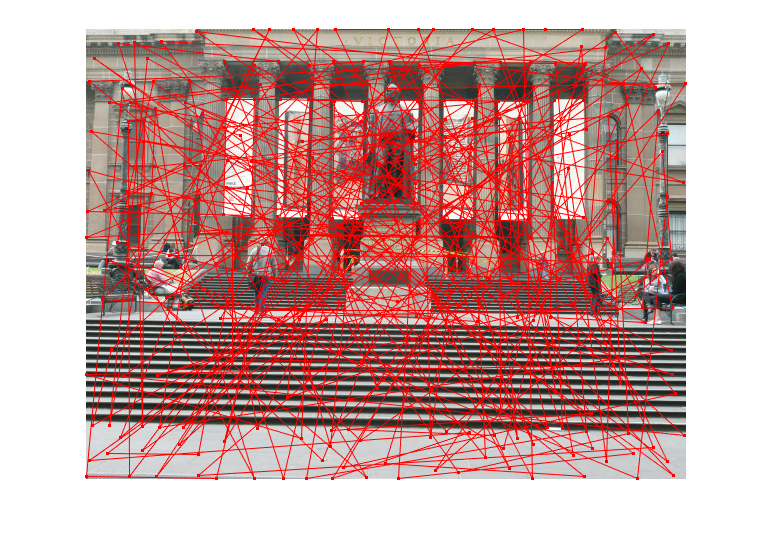
\includegraphics[width=275]{outputimages/ANMS/ANMS5.png}
\end{center}

\section[]{Feature Descriptor}

\subsection{This is a B head this is a B head this is a B head this is a B head this is a B~head}
\subsubsection{This is a C head this is a C head this is a C head this is a C head}


\section{Feature Matching}

List in \LaTeX{} can be of three types: enumerate, itemize and description.
In each environments, new entry is added via the \verb+\item+ command.
Enumerate creates numbered lists, itemize creates bulleted lists and
description creates description lists.
\begin{enumerate}[1.]
\item First item in the number list.
\item Second item in the number list.
\item Third item in the number list.
\end{enumerate}
List in \LaTeX{} can be of three types: enumerate, itemize and description.
In each environments, new entry is added via the \verb+\item+ command.
\begin{itemize}
\item First item in the bullet list.
\item Second item in the bullet list.
\item Third item in the bullet list.
\end{itemize}


\section{RANSAC to estimate Robust Homography}

Equations in \LaTeX{} can either be inline or on-a-line by itself. For
inline equations use the \verb+$...$+ commands. Eg: The equation
$H\psi = E \psi$ is written via the command $H \psi = E \psi$.



\section{Cylinirical Projection}

\begin{figure}[t]%
\FIG{\includegraphics[width=.75\columnwidth]{Fig}}
{\caption{This is an example of caption this is an example of caption  this is an example of caption this is an example of caption}
\label{fig1}}
\end{figure}

\section{Blending Images}



\begin{table}[t]
\tabcolsep=0pt%
\TBL{\caption{Tables which are too long to fit,
should be written using the ``table*'' environment\label{tab2}}}
{\begin{fntable}
\begin{tabular*}{\textwidth}{@{\extracolsep{\fill}}lcccccc@{}}\toprule%
 & \multicolumn{3}{@{}c@{}}{\TCH{Element 1}}& \multicolumn{3}{@{}c@{}}{\TCH{Element 2\smash{\footnotemark[1]}}}
 \\\cmidrule{2-4}\cmidrule{5-7}%
\TCH{Project} & \TCH{Energy} & \TCH{$\boldsymbol{\sigma_{\text{calc}}}$} & \TCH{$\boldsymbol{\sigma_{\text{expt}}}$} &
\TCH{Energy} & \TCH{$\boldsymbol{\sigma_{\text{calc}}}$} & \TCH{$\boldsymbol{\sigma_{\text{expt}}}$} \\\midrule
\TCH{Stage 3}&990 A &168 &47$\pm$12 &78 A &66 &39$\pm$10\\
{\TCH{Stage 4}}&500 A &961 &22$\pm$10 &90 A &68 &92$\pm$40\\
\botrule
\end{tabular*}%
\footnotetext[]{{Note:} This is an example of table footnote this is an example of table footnote this is an example of table footnote this is an example of~table footnote this is an example of table footnote}
\footnotetext[1]{This is an example of table footnote}%
\end{fntable}}
\vspace*{7pt}
\end{table}



\section{Conclusion}

Some Conclusions here.



\begin{Backmatter}
\begin{thebibliography}{}
\bibitem[Ananin and Mironov (2000)]{bib1}
{Ananin, Beth, and Mironov, Antony}. 2000. ``The moduli space of $2$-dimensional algebras'', \textit{Comm. Algebra} {28}(9),  {4481}--{4488}.

\bibitem[Bai and Meng (2001)]{bib2}
{Bai, Clifton, and Meng, Dyck}. 2001. ``The classification of Novikov algebras in low dimension'',  \textit{J. Phys. A: Math. Gen.} {34}, {1581}--{1594}.

\bibitem[Ca\~{n}ete and Khudoyberdiyev (2013)]{bib3}
{Ca\~{n}ete, Enderson, and Khudoyberdiyev, Angus}. 2013. ``The classification of $4$-dimensional Leibniz algebras'',  \textit{Linear Algebra and its Applications}  {439}(1), {273}--{288}.

\bibitem[Goze and Remm (2011)]{bib4}
{Goze, Michael, and Remm, Edward}. 2011.  ``$2$-dimensional algebras'',  \textit{Afr. J. Math. Phys.} {10}(1),  {81}--{91}.

\bibitem[Petersson (2000)]{bib5}
{Petersson, Hentry}. 2000. ``The classification of two-dimensional nonassociative algebras'',  \textit{Results Math} {37}, no. 1-2,  {120}--{154}.

\end{thebibliography}

\end{Backmatter}
\end{document}
